\documentclass[conference]{IEEEtran}
\IEEEoverridecommandlockouts
\usepackage{cite}
\usepackage{amsmath,amssymb,amsfonts}
\usepackage{algorithmic}
\usepackage{graphicx}
\usepackage{textcomp}
\usepackage{xcolor}
\usepackage{booktabs}
\usepackage{subcaption}
\usepackage{url}
\usepackage[colorlinks=true, linkcolor=black, urlcolor=blue, citecolor=black]{hyperref}

\def\BibTeX{{\rm B\kern-.05em{\sc i\kern-.025em b}\kern-.08em
    T\kern-.1667em\lower.7ex\hbox{E}\kern-.125emX}}
\begin{document}

\title{Unmasking Fraud in Transaction Networks: Harnessing Heterogeneous Graph Neural Networks for Enhanced Detection\\
}

\author{\IEEEauthorblockN{ Kanishk Goel}
\IEEEauthorblockA{\textit{Department of Data Science} \\
\textit{George Washington University}\\
Washington DC, USA \\
}
\and
\IEEEauthorblockN{Amir Hossein Jafari}
\IEEEauthorblockA{\textit{Department of Data Science} \\
\textit{George Washington University}\\
Washington DC, USA \\
}
}

\maketitle

\begin{abstract}
Credit card fraud pose a significant threat to global financial systems. They lose billions of dollars annually. Traditional machine learning techniques such as Random Forests and XGBoost have demonstrated effectiveness in fraud detection. However, they often fail to capture the complex interdependencies among entities involved in transactions. This paper explores the efficacy of Graph Neural Networks motivated by recent advances in graph-based learning. We focus on Heterogeneous Graph Convolutional Networks for enhanced credit card fraud detection.

We conduct a comparative study between classical ML models and GNNs using a synthetically generated credit card transaction dataset. Over one million records simulate interactions between customers, merchants, and transactions. The graph-based structure these entities as distinct node types connected by meaningful edges. We implement the GNN framework using PyTorch Geometric and evaluate the models using the F1-score to account for class imbalance.

Experimental results demonstrate that GNNs outperform traditional ML classifiers by leveraging relational information and neighbourhood context. They detect fraudulent patterns, especially when we have more embeddings and fewer meaningful features. This work reinforces the potential of graph-based learning as a powerful approach for high-volume and relationally rich transaction networks.


\end{abstract}

\begin{IEEEkeywords}
Credit card, fraud detection, HeteroGCN, GNN, Node classification
\end{IEEEkeywords}

\section{Introduction}

In the digital economy, the rapid adoption of online transactions and plastic money has increased the prevalence of credit card fraud affecting consumers, businesses, and financial institutions \cite{chaudhary2012review}. The nature of credit card fraud is constantly evolving, such as phishing, counterfeit cards, identity theft, and unauthorized online transactions \cite{xuan2018random}. Fraudulent activities significantly erode user trust, increase operational costs, and introduce regulatory challenges despite forming a small proportion of all transactions \cite{sailusha2020ml}. 

Traditionally, fraud detection relied on rule-based systems and manual investigations, which are now rendered inadequate by the scale and velocity of modern digital transactions. Recent years have seen the deployment of machine learning (ML) methods such as Logistic Regression, Decision Trees, and ensemble models like Random Forests and XGBoost for fraud detection \cite{awoyemi2017comparative, xuan2018random}. These models offer promising accuracy but treat transactions as isolated events and fail to exploit relational information between entities involved in transactions.

Our work investigates Graph Neural Networks to address this limitation. GNNs model transactions as interactions within a network of entities such as users, merchants, and transactions. Such capabilities make them well-suited for detecting subtle anomalies in transaction behaviour indicative of fraud.

In this study, we propose a comparative evaluation of traditional ML models—Random Forests and XGBoost—against a GNN-based architecture implemented using PyTorch Geometric. We utilize a large-scale, synthetically \cite{data_generation} generated dataset \cite{dataset1} simulating over 1.3 million transactions and perform evaluations using F1-score to address the challenge of class imbalance. The objectives of this research are:

\begin{itemize}
    \item To design a heterogeneous graph-based model capturing relationships between transactions, users, and merchants.
    \item To benchmark the performance of GNNs against state-of-the-art ML classifiers on a realistic fraud detection task.
    \item To assess the potential of GNNs in modelling contextual information that improves fraud detection accuracy and interpretability.
\end{itemize}

Our research contributes toward building more robust and scalable fraud detection systems capable of early detection and mitigation of financial risks by integrating transaction context through graph structures.


\section{Related work}

Credit card fraud detection has been a crucial application domain for machine learning which has grown in the last decade. Traditional supervised learning approaches have been widely employed due to their interpretability and strong baseline performance on structured tabular datasets \cite{awoyemi2017comparative,xuan2018random} with rich features. More recently, Graph Neural Networks (GNNs) have emerged as a powerful alternative due to their ability to model and leverage complex relational information among entities \cite{cheng2025gnnreview}. We organise this section into two parts: classical machine learning approaches and graph-based methods, critically evaluating their strengths, limitations, and highlighting how our work advances the state of the art.

\subsection{Machine Learning Approaches}

Classical machine learning models have formed the backbone of anomaly detection systems. Logistic Regression, Decision Trees, Random Forests, and XGBoost have been used extensively due to their ease of implementation and good evaluation scores in high-dimensional feature spaces \cite{chaudhary2012review,ieee1297040}. These models typically operate on individual transaction records represented in a flat feature vector format.

Random Forest is effective in reducing overfitting through bootstrapped aggregation of multiple decision trees \cite{xuan2018random}. XGBoost improves over Random Forests by iteratively boosting weak learners and has demonstrated superior performance in several studies \cite{IEEE9719580}. However, both models suffer from the inability to capture interactions beyond engineered features. They often miss higher-order relational patterns between users and merchants that are critical for fraud detection.

Moreover, as our work suggests, these models do not account for contextual signals such as shared card usage across merchants or sudden behavioural shifts in merchant-customer interactions. Ensemble methods can marginally improve predictive power but they still treat samples independently and lack the capacity to model transactional dependencies.

\subsection{Graph Based Approach}

Graph Neural Networks have emerged as a powerful deep learning paradigm for learning graphical data. This allows models to exploit the underlying structure of financial transaction networks. GNNs address key disadvantages of classical models by exploiting the relational structure inherent in financial transactions. They excel at modelling the complex, dynamic relationships between heterogeneous entities - customers, merchants, and transactions. Graphs are especially effective in uncovering fraud rings and hidden behavioural patterns that may not be evident in tabular representations \cite{cheng2025gnnreview}. Each transaction can be viewed as an affair between a user and a merchant, and these often participate in the whole network. \cite{IEEE9667674}. GNNs propagate information between nodes using message-passing mechanisms, enabling the model to learn complex patterns beyond what flat features can capture.

Graph Convolutional Networks apply spectral convolutions over node neighbourhoods and effectively learn representations by aggregating information from adjacent nodes. GCNs are prone to over-smoothing with increasing depth \cite{cheng2025gnnreview}. In contrast, Graph Attention Networks (GATs) assign adaptive weights to neighbours to focus on more relevant parts of the graph \cite{IEEE9906987}.

Lately, some papers have explored the use of Heterogeneous graphs to handle multiple node and edge types. These models are particularly suited to credit card fraud detection, where nodes represent transactions, users, and merchants, and edges encode different relation types. Our approach extends prior efforts by constructing a real-world heterogeneous graph and using PyTorch Geometric frameworks to implement scalable GNN architectures.

In summary, our work is distinguished by a systematic benchmarking against classical methods, use of the Pytorch Geometric library, and deployment on a richly featured synthetic dataset. This comparative analysis offers new insights into the efficacy and trade-offs of adopting GNNs for real-world financial fraud detection systems.



\section{Methodology}
%add content

\subsection{Machine Learning Models}\label{AA}
For the comparative analysis, we set baselines with several machine learning models - Logistic Regression, Decision Trees, Random Forest and XGBoost for model evaluation. As the data is in tabular format, classical modelling makes sense. These models are trained on structured tabular features extracted from transactions, users, and merchants.

We evaluate the following supervised classification models:


\subsubsection{Logistic Regression}
Logistic Regression is a linear model that estimates the probability of a binary outcome using the logistic (sigmoid) function as shown below: 
\begin{equation}
    \hat{y} = \frac{1}{1 + e^{-(\mathbf{w}^\top \mathbf{x} + b)}}
    \label{eq:logistic}
\end{equation}
where $\mathbf{x}$ is the input feature vector, $\mathbf{w}$ denotes the model weights, $b$ is the bias term, and $\hat{y}$ represents the predicted probability of fraud.


The model is trained by minimising the binary cross-entropy loss:

\begin{equation}
    \mathcal{L} = -\frac{1}{N} \sum_{i=1}^{N} \left[y_i \log \hat{y}_i + (1 - y_i) \log(1 - \hat{y}_i)\right]
\end{equation}
 It is suitable for linearly separable data.


\subsubsection{Decision Tree}
Decision Trees are non-parametric models that recursively partition the input space into class-pure regions. At each split, the algorithm chooses the feature and threshold that minimise an impurity measure and maximise information gain. For each node, we used Gini impurity as impurity measure:

\begin{equation}
    \text{Gini}(S) = 1 - \sum_{c=1}^{C} p(c)^2
    \label{eq:gini}
\end{equation}
where $C$ is the number of classes and $p(c)$ is the proportion of class $c$ in node $S$.

Alternatively, the splitting criterion can be based on \textit{entropy} and \textit{information gain}. The entropy of a node $S$ is defined as:
\begin{equation}
    \text{Entropy}(S) = -\sum_{c=1}^{C} p(c) \log_2 p(c)
    \label{eq:entropy}
\end{equation}

The \textit{information gain} from splitting on attribute $A$ is given by:
\begin{equation}
    \text{IG}(S, A) = \text{Entropy}(S) - \sum_{v \in \text{Values}(A)} \frac{|S_v|}{|S|} \, \text{Entropy}(S_v)
    \label{eq:infogain}
\end{equation}
where $S_v$ is the subset of $S$ where attribute $A$ has value $v$, and $|S_v|/|S|$ is the proportion of samples in that subset.

Decision trees are prone to overfitting without regularisation.

\subsubsection{Random Forest}
To avoid high variance, we use Random Forests. These are ensemble models that aggregate the predictions of multiple decision trees trained on bootstrapped subsets of data and random subsets of features. We use an ensemble of $T$ decision trees:
\begin{equation}
    \hat{y} = \frac{1}{T} \sum_{t=1}^{T} h_t(\mathbf{x})
\end{equation}

where each $h_t$ is a decision tree trained. The final prediction is made by majority voting in classification tasks. Random Forests are robust to noise and capable of capturing nonlinear relationships.


\subsubsection{XGBoost}
XGBoost is a scalable and regularised boosting method that trains an ensemble of models sequentially, where each new model attempts to correct the residuals of the previous ensemble. It builds an ensemble of additive trees using gradient boosting:
\begin{equation}
    \hat{y}_i^{(t)} = \hat{y}_i^{(t-1)} + \eta f_t(\mathbf{x}_i)
    \label{eq:xgb-update}
\end{equation}
where $f_t$ is the $t$-th regression tree, and $\eta$ denotes the learning rate. The model minimises a regularised loss function defined as:
\begin{equation}
    \mathcal{L}^{(t)} = \sum_{i=1}^{N} l(y_i, \hat{y}_i^{(t)}) + \sum_{t=1}^{T} \Omega(f_t)
    \label{eq:regularized-loss}
\end{equation}
where $l(y_i, \hat{y}_i^{(t)})$ is the prediction loss and $\Omega(f_t)$ is the regularization term for tree $f_t$. The regularisation function is given by:
\begin{equation}
    \Omega(f) = \gamma T + \frac{1}{2} \lambda \sum_{j=1}^{T} w_j^2
    \label{eq:regularization}
\end{equation}
where $T$ is the number of leaves in the tree, $w_j$ is the score on the $j$-th leaf, $\gamma$ is the complexity penalty for each leaf, and $\lambda$ controls the $L_2$ regularization on leaf weights.




\subsection{Graph Neural Networks}
\subsubsection{Graph Construction}
As the problem statement is to predict fraud transactions, one node type will be transaction. We also have to consider the user and merchant because they act as two entities between which the transaction occurs. This is why we used Heterogeneous graphs. For each node type we have a primary id. Credit card numbers are used as user id, and we add mappings for both unique transactions and unique merchants. 
The heterogeneous graph is constructed using PyG's \texttt{HeteroData} object. The graph schema is defined as follows:
\begin{equation}
    \mathcal{G} = (\mathcal{V}, \mathcal{E}, \mathcal{T}_v, \mathcal{T}_e)
    \label{eq:hetero-graph}
\end{equation}
where $\mathcal{V}$ denotes the set of nodes, $\mathcal{E}$ the set of edges, $\mathcal{T}_v$ the set of node types (e.g., \texttt{transaction}, \texttt{user}, \texttt{merchant}), and $\mathcal{T}_e$ the set of edge types that define the relationships between nodes.

Each node type $t \in \mathcal{T}_v$ has an associated feature matrix $X^{(t)} \in \mathbb{R}^{N_t \times d_t}$, where $N_t$ is the number of nodes of type $t$ and $d_t$ is the feature dimension for that node type.

Specifically, the feature matrices for each node type are as follows:
\begin{itemize}
    \item For \texttt{transaction} nodes: $X^{(\texttt{transaction})} \in \mathbb{R}^{N_T \times 8}$,
    \item For \texttt{user} nodes: $X^{(\texttt{user})} \in \mathbb{R}^{N_U \times 4}$,
    \item For \texttt{merchant} nodes: $X^{(\texttt{merchant})} \in \mathbb{R}^{N_M \times 3}$.
\end{itemize}

The graph includes bidirectional edge types defined as:
\begin{itemize}
    \item (\texttt{transaction}, \texttt{transaction\_to\_user}, \texttt{user})
    \item (\texttt{user}, \texttt{user\_to\_transaction}, \texttt{transaction})
    \item (\texttt{transaction}, \texttt{transaction\_to\_merchant}, \texttt{merchant})
    \item (\texttt{merchant}, \texttt{merchant\_to\_transaction}, \texttt{transaction})
    \item (\texttt{user}, \texttt{user\_to\_merchant}, \texttt{merchant})
    \item (\texttt{merchant}, \texttt{merchant\_to\_user}, \texttt{user})
\end{itemize}

The label for fraud classification is defined on the \texttt{transaction} nodes as:
\begin{equation}
    \mathbf{y}^{(\texttt{transaction})} \in \{0, 1\}^{N_{\texttt{transaction}}}
    \label{eq:label}
\end{equation}
indicating whether each transaction is fraudulent ($1$) or not ($0$).

\begin{figure}[htbp]
    \centering
    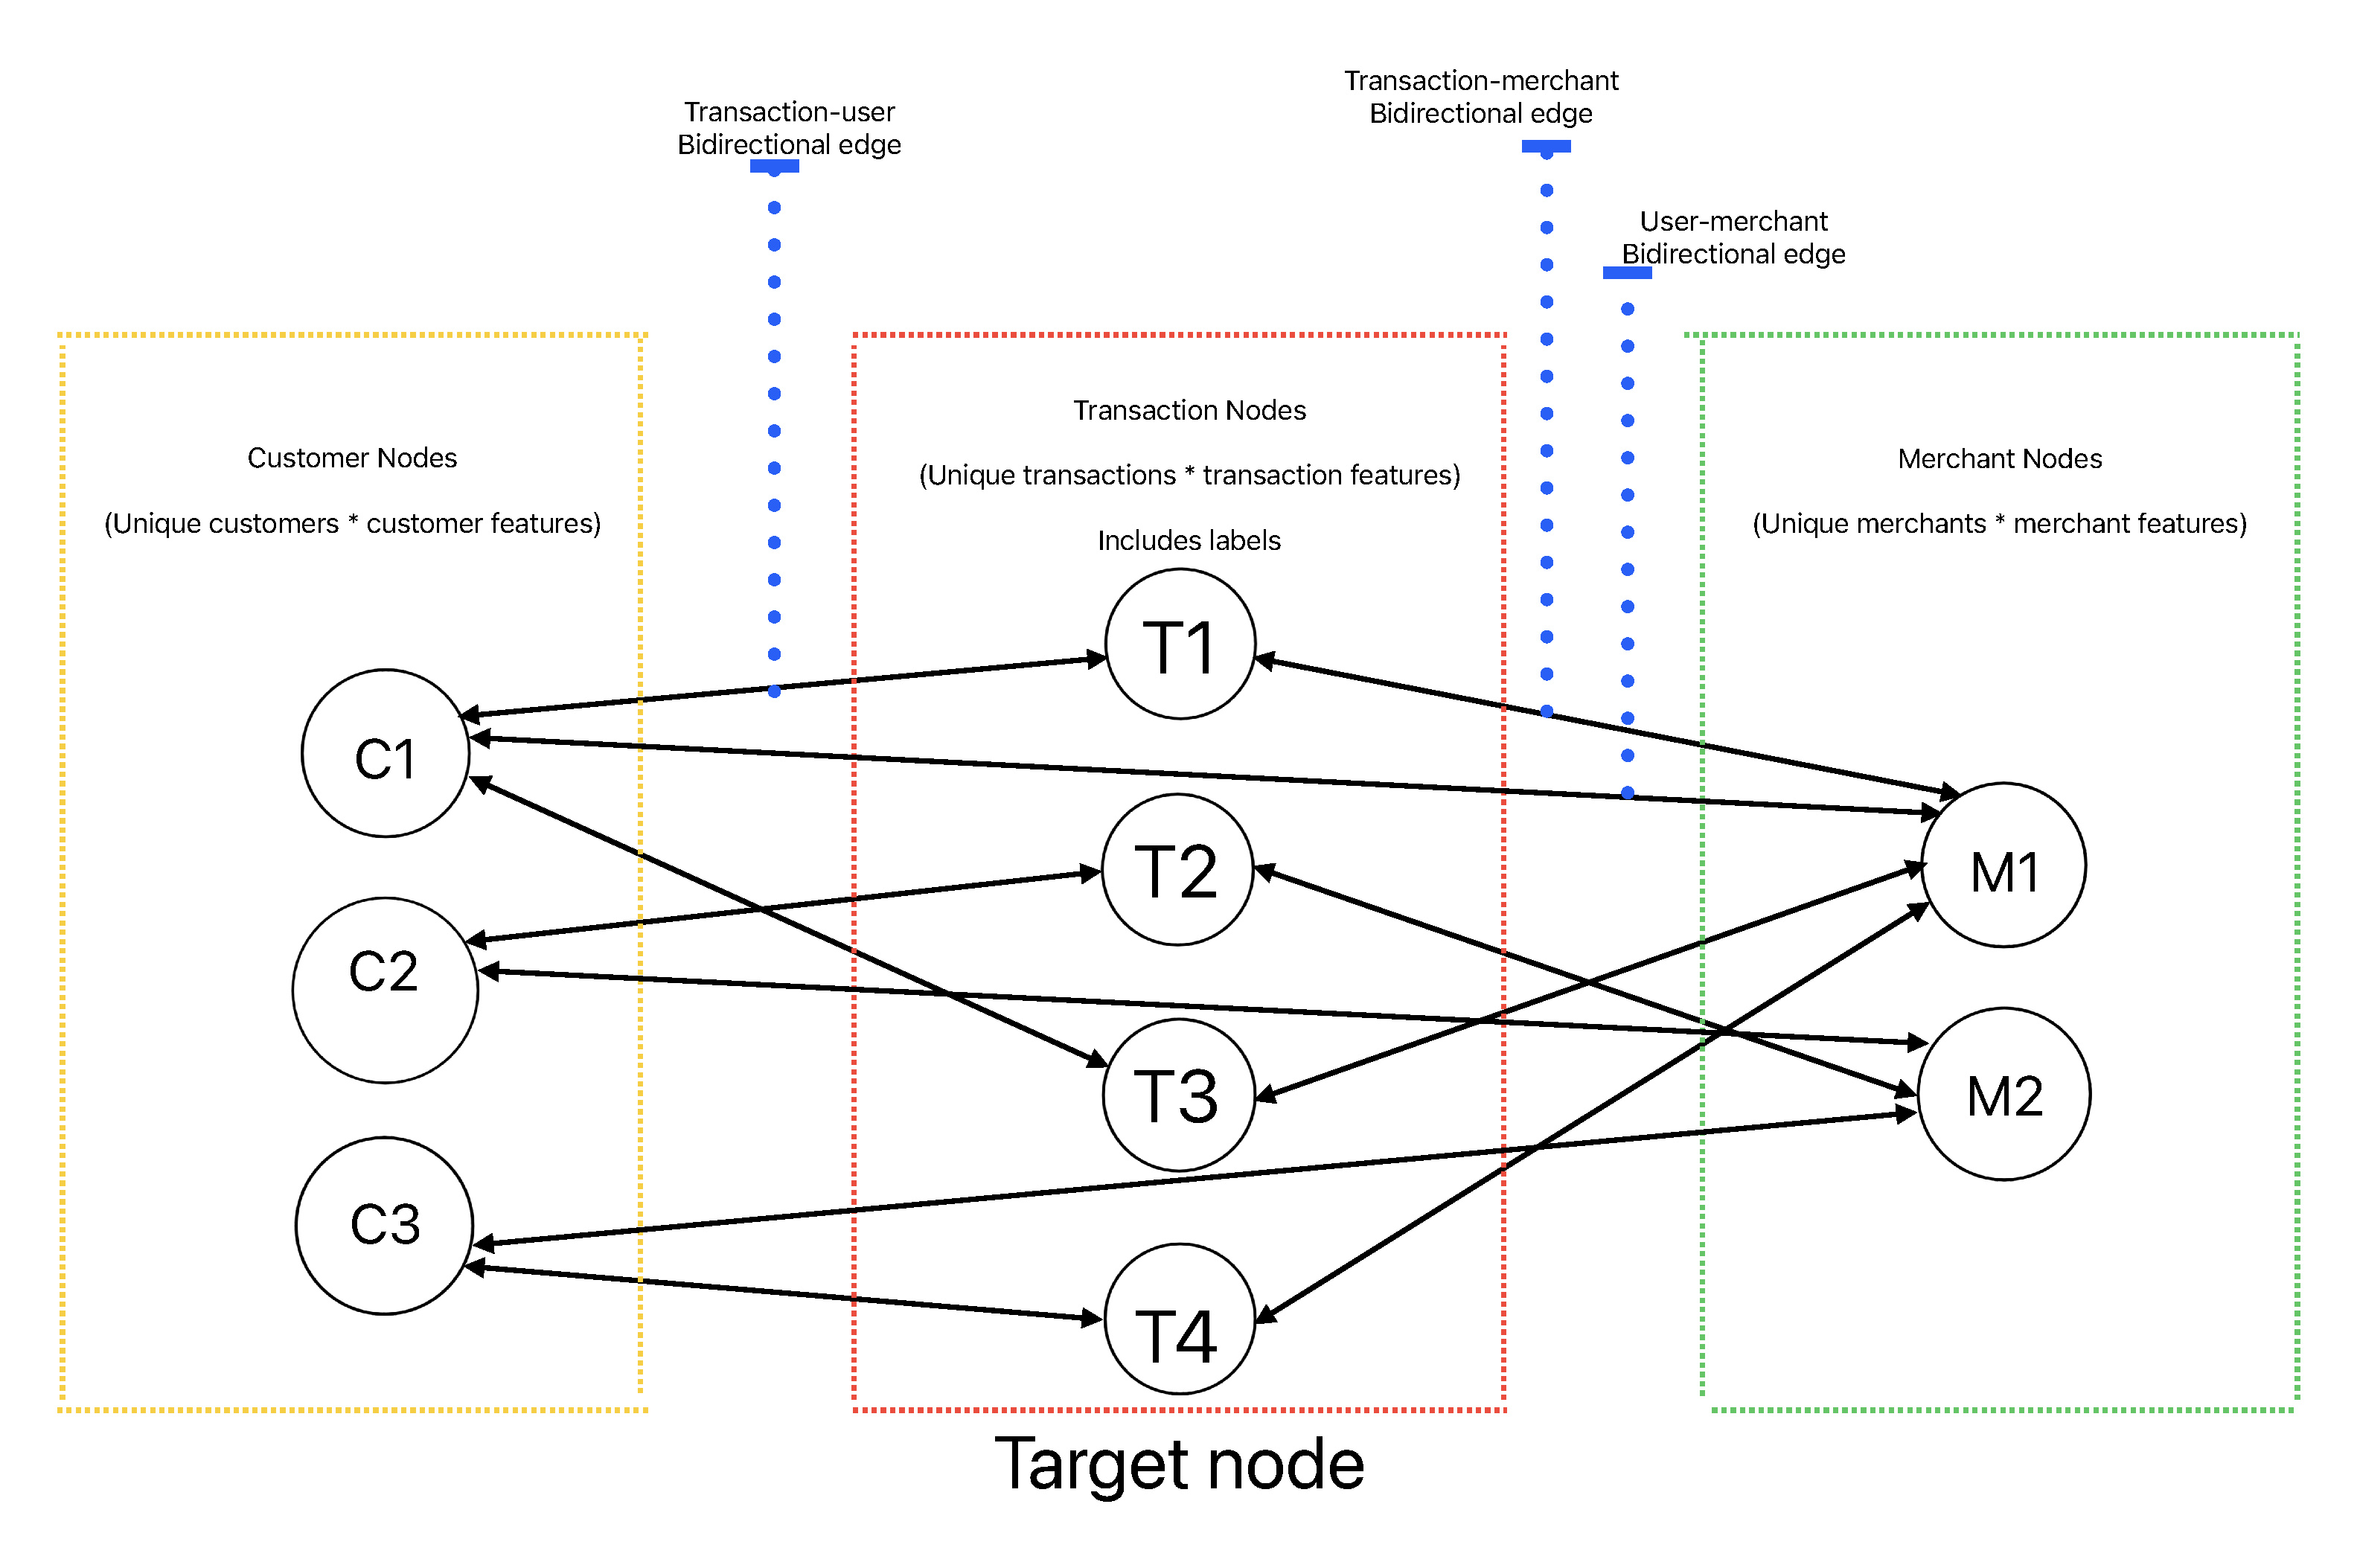
\includegraphics[width=0.4\textwidth, keepaspectratio]{Graph structure.pdf}
    \caption{Heterogenous graph structure}
    \label{fig:gnn-layer}
\end{figure}


\subsubsection{HeteroGCN Architecture}

We implement a \textbf{Heterogeneous Graph Neural Network (HeteroGNN)} using PyTorch Geometric (PyG) for the task of fraud detection. The model leverages message passing through type-specific GraphSAGE layers within the \texttt{HeteroConv} framework.

\paragraph{Input Projection}
Since node feature dimensions vary across types, input projection layers are applied to project all features into a shared hidden space of dimension $d$. The initial embedding for a node $v$ of type $t$ is computed as:
\begin{equation}
    h_v^{(0)} = W_{\text{proj}}^{(t)} x_v, \quad \forall v \in \mathcal{V}_t
    \label{eq:input-projection}
\end{equation}
where $x_v \in \mathbb{R}^{d_t}$ is the original feature vector, $W_{\text{proj}}^{(t)} \in \mathbb{R}^{d_t \times d}$ is the type-specific projection matrix, and $h_v^{(0)}$ is the initial node embedding.

\paragraph{Message Passing}
For the message passing stage, we utilise the \texttt{HeteroConv} operator, which aggregates relation-specific messages through \texttt{SAGEConv} layers. The hidden representation of node $i$ at layer $l+1$ is computed as:
\begin{equation}
    h_i^{(l+1)} = \sigma \left( \sum_{r \in \mathcal{R}} \texttt{SAGEConv}_r(h_i^{(l)}, \{ h_j^{(l)} : j \in \mathcal{N}_r(i) \}) \right)
    \label{eq:message-passing}
\end{equation}
where $\mathcal{R}$ is the set of edge types, $\mathcal{N}_r(i)$ represents neighbors of node $i$ under relation $r$, $\texttt{SAGEConv}_r$ denotes the GraphSAGE convolution for relation $r$, and $\sigma$ is the LeakyReLU activation function. The \texttt{HeteroConv} operator sums over contributions from all relations.

\paragraph{Output Layer and Classification}
A final linear classifier is applied to the embeddings of the target \texttt{transaction} nodes:
\begin{equation}
    \hat{y}_i = \text{softmax}(W_{\text{out}} \cdot h_i^{(L)})
    \label{eq:output}
\end{equation}
where $W_{\text{out}}$ is the output weight matrix and $L$ is the number of GNN layers.

\paragraph{Loss Function:}
We optimise the model using the \texttt{AdamW} optimiser with L2 regularisation. The objective is the standard cross-entropy loss:
\begin{equation}
    \mathcal{L} = -\log \left( \frac{\exp(z_{i,y_i})}{\sum_{j} \exp(z_{i,j})} \right)
    \label{eq:crossentropy}
\end{equation}
where $z_{i,j}$ denotes the $j$-th logit for node $i$, and $y_i$ is the ground-truth class.

\begin{figure}[htbp]
    \centering
    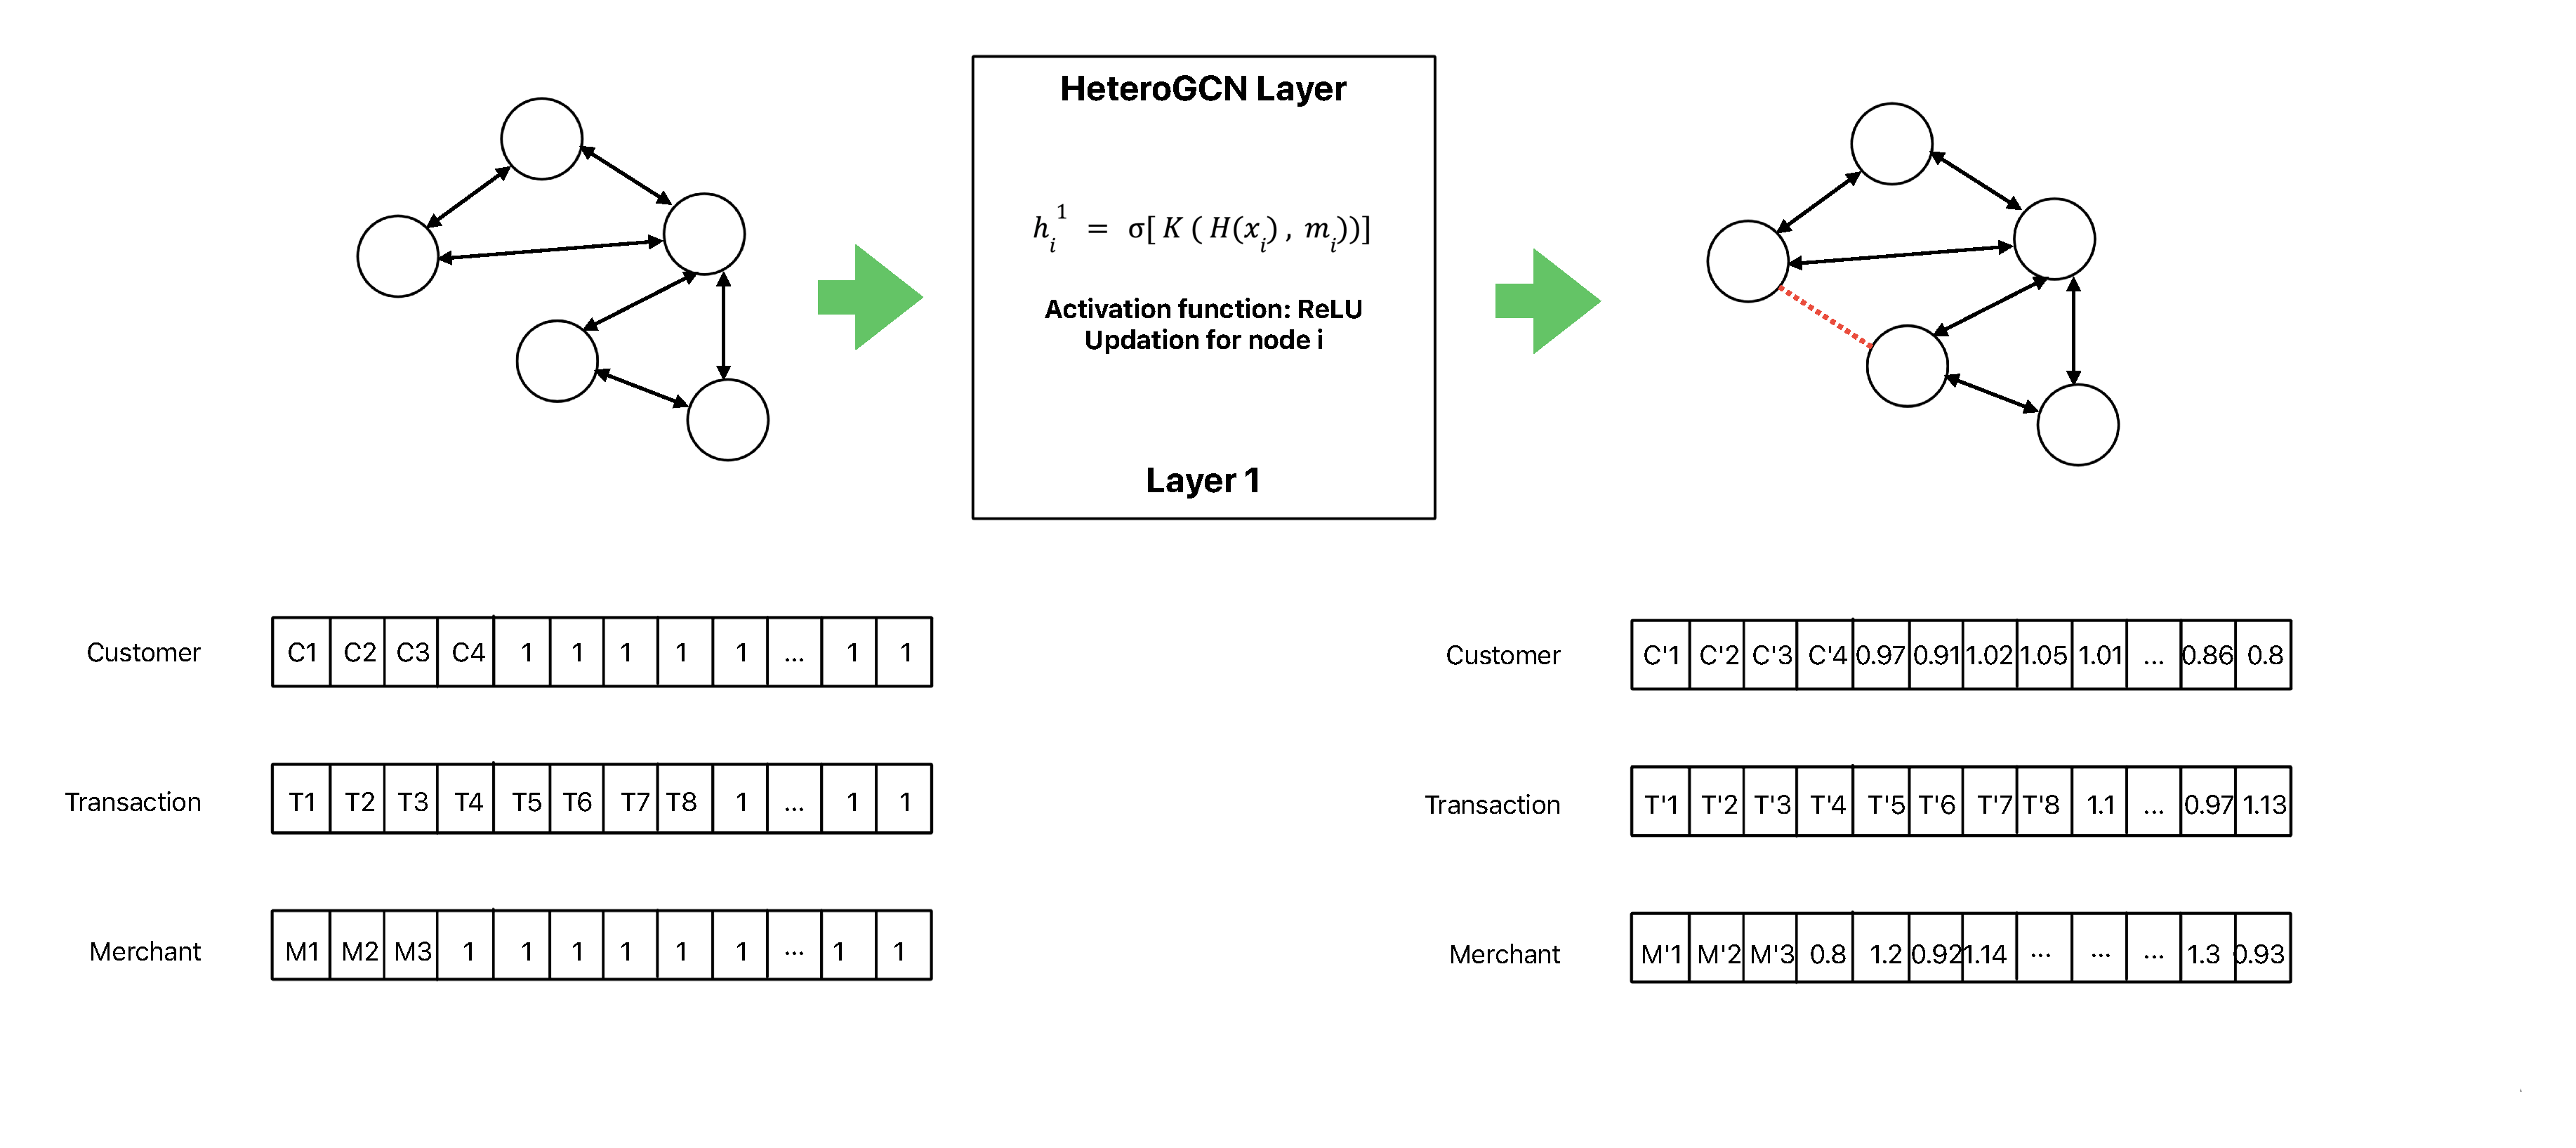
\includegraphics[width=0.4\textwidth, keepaspectratio]{Model_arch.pdf}
    \caption{HeteroGNN model architecture}
    \label{fig:gnn-layer}
\end{figure}

\section{Experimentation}
\subsection{Dataset}
Two synthetically generated datasets are utilised to develop and evaluate the fraud detection models. Both datasets reflect realistic financial transaction behaviour, encompassing legitimate and fraudulent activities.

Dataset 1 consists of simulated credit card transactions spanning the period from January 1, 2019 to December 31, 2020. It includes transactions conducted by 1000 unique customers interacting with 800 merchants. The data was generated using the Sparkov Data Generation tool \cite{dataset1}.

Each record contains temporal, geographical, and behavioural features such as transaction date and time, merchant category, transaction amount, cardholder demographic information (e.g., gender, city, state, zip code, latitude/longitude), and a binary fraud indicator. The key columns include:
\begin{itemize}
    \item trans\_date\_trans\_time
    \item cc\_num
    \item merchant
    \item category
    \item amt
    \item city
    \item state
    \item dob
    \item merch\_lat
    \item merch\_long
    \item is\_fraud
\end{itemize}


Dataset 2 was synthetically generated using a Python pipeline \cite{data_generation} to simulate a diverse set of transactional patterns across multiple sectors. It emulates global financial behaviour by incorporating multiple currencies, geographic regions, and consumer profiles. This dataset is designed to support robust exploratory analysis and training of fraud detection models.

The data spans various merchant categories (e.g., retail, entertainment, travel, healthcare), and captures metadata such as device type, currency, country, transaction time, and city size. It also includes indicators for transaction risk and contextual signals such as distance from home and weekend occurrence.

Representative features include:
\begin{itemize}
    \item transaction\_id
    \item timestamp
    \item amount
    \item currency
    \item country
    \item city\_size
    \item merchant\_category
    \item device
    \item high\_risk\_merchant
    \item weekend\_transaction
    \item is\_fraud
\end{itemize}


\subsection{Data Preprocessing}

To ensure the dataset is suitable for training both traditional machine learning and graph-based models, we construct a dedicated preprocessing pipeline. This pipeline transforms raw transactional data into a structured format with clean, informative, and numerically encoded features. It accepts a DataFrame as input and performs a sequence of transformations to extract features essential for downstream model training.

\subsubsection{Temporal Feature Engineering}

The timestamp column is first converted using the \texttt{pd.to\_datetime()} function. From this, temporal components such as the hour of the day and the day of the month are extracted. To preserve the cyclic nature of time—e.g., hours 23:00 and 00:00 being close—sine and cosine transformations are applied:

\begin{equation}
    \text{day\_sin} = \sin\left( \frac{2\pi \cdot \text{day}}{31} \right)
    \label{eq:day-sin}
\end{equation}

\begin{equation}
    \text{day\_cos} = \cos\left( \frac{2\pi \cdot \text{day}}{31} \right)
    \label{eq:day-cos}
\end{equation}


These transformations allow the model to capture temporal proximity in a continuous, differentiable space.

\subsubsection{Categorical Encoding}

Categorical columns such as \texttt{merchant category} are encoded using a combination of one-hot encoding, label encoding, and target encoding depending on the context and cardinality of the feature. This enhances the ability of both tree-based and neural models to utilize categorical information effectively.

\subsubsection{Entity ID Mapping}

To enable graph-based learning, string-based identifiers are mapped to unique integer indices. Specifically, \texttt{transaction\_id}, \texttt{merchant}, and \texttt{cc\_num} are encoded as follows:
\begin{itemize}
    \item \texttt{transaction\_id} is mapped to sequential transaction indices,
    \item \texttt{merchant} is mapped to \texttt{merchant\_id},
    \item \texttt{cc\_num} is mapped to \texttt{user\_id}.
\end{itemize}

Additionally, irrelevant or redundant columns such as \texttt{first}, \texttt{last}, \texttt{street}, and \texttt{day\_period} are dropped to ensure data consistency and eliminate noise.

\begin{figure}[htbp]
    \centering
    \begin{subfigure}{0.45\columnwidth}
        \centering
        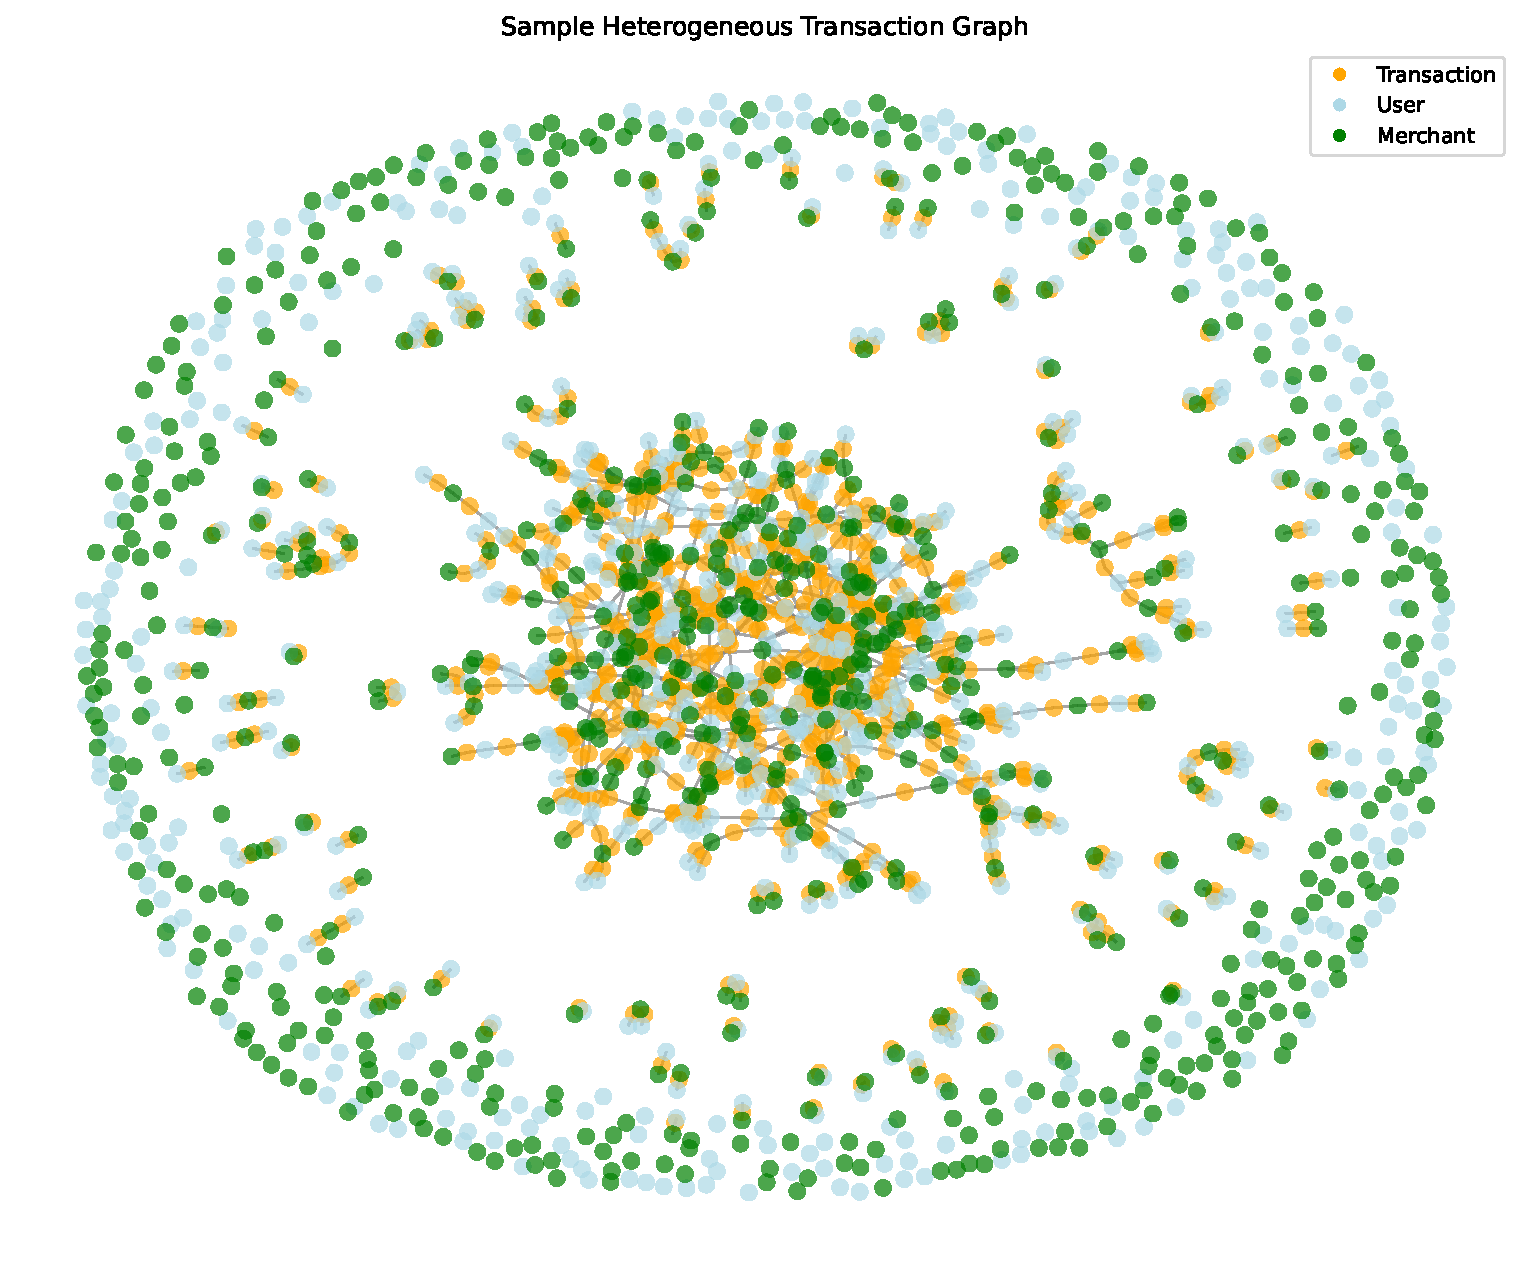
\includegraphics[width=\linewidth]{Graph DS1.pdf}
        \caption{Dataset 1}
        \label{fig:graph-ds1}
    \end{subfigure}
    \hfill
    \begin{subfigure}{0.45\columnwidth}
        \centering
        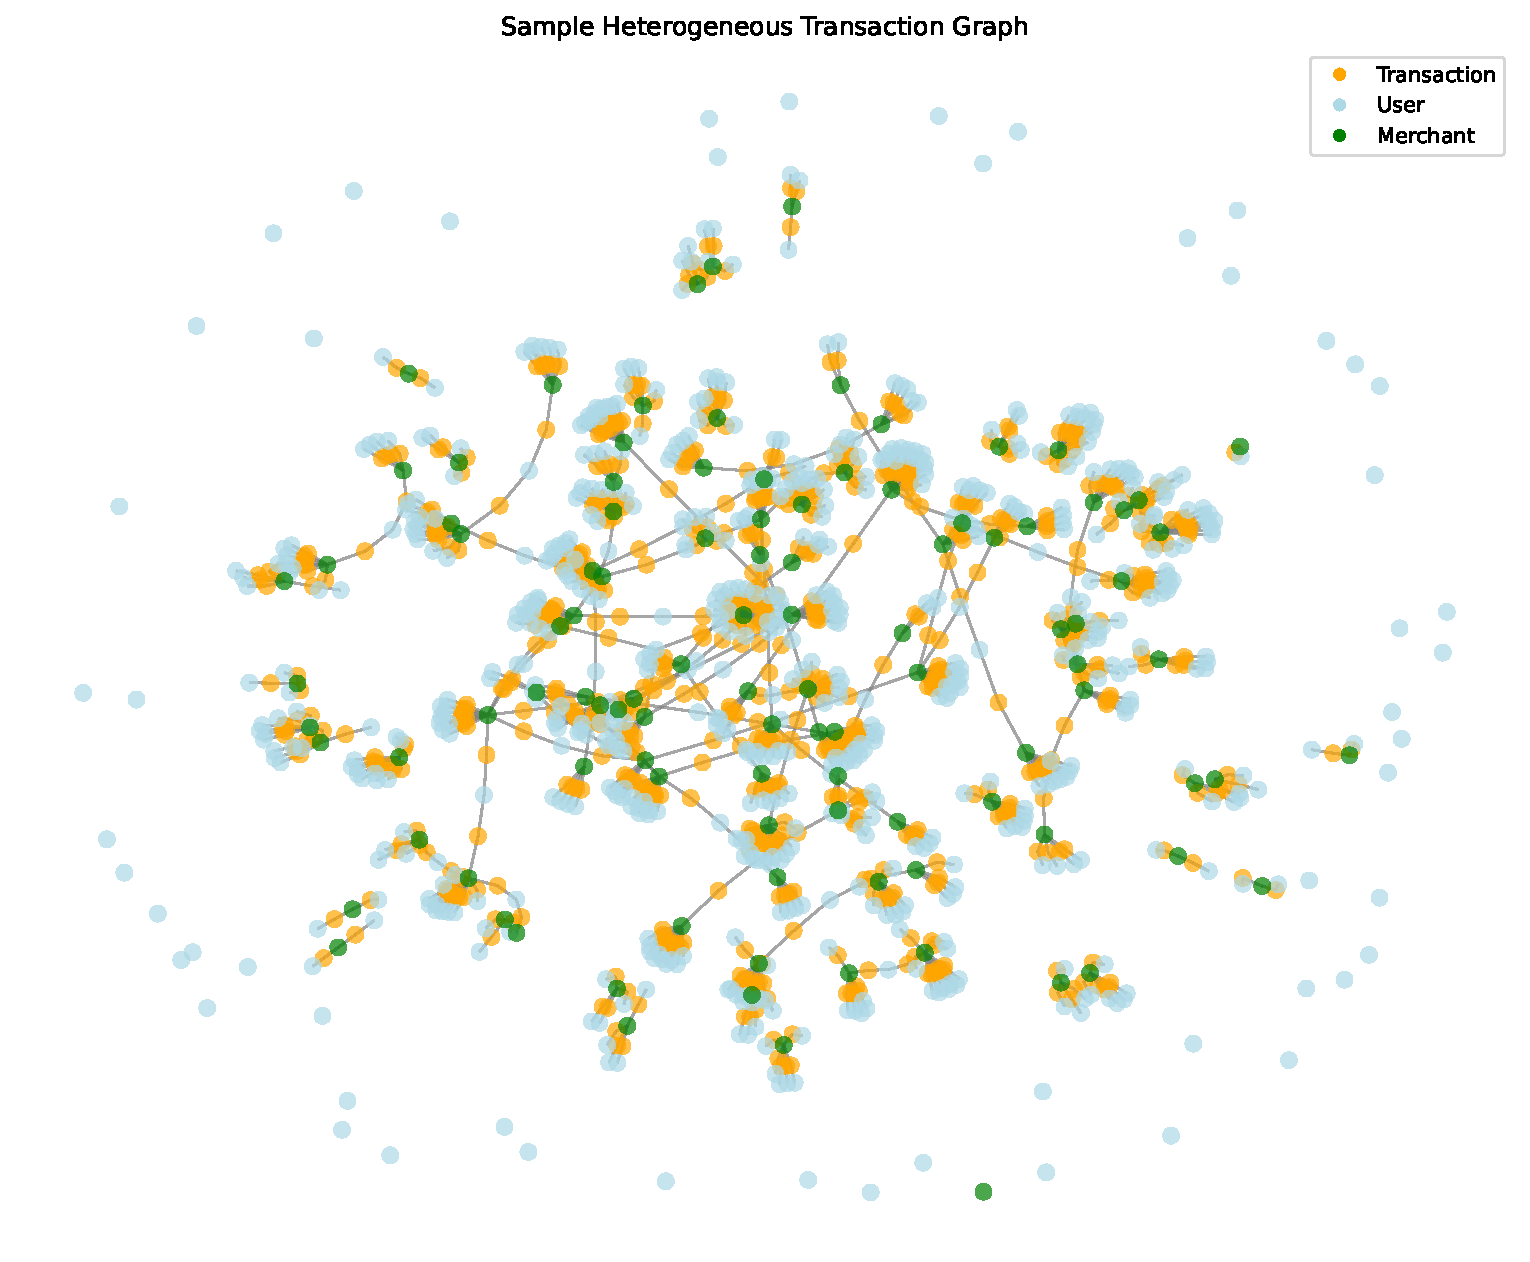
\includegraphics[width=\linewidth]{Graph DS2.pdf}
        \caption{Dataset 2}
        \label{fig:graph-ds2}
    \end{subfigure}
    
    \caption{Sample Graph Representations for Dataset 1 and 2.}
    \label{fig:graph-datasets}
\end{figure}



\subsection{Experimental Setup}

We constructed a heterogeneous graph with features extracted from the preprocessed data using PyTorch Geometric’s \texttt{HeteroData} structure. Edges were added bidirectionally to model relations such as \texttt{user-to-transaction}, \texttt{merchant-to-transaction}, and self-loops on transaction nodes. The graph was split into training and validation sets using a stratified 80/20 split on the fraud label.

The GNN model employed a multi-relational message-passing architecture via the \texttt{HeteroConv} module, with GraphSAGE layers specific to each edge type. The following hyperparameters were used during training: a hidden size of 32, output size of 2 for binary classification, 4 message-passing layers, target node type set to \texttt{transaction}, and sum-based aggregation. The learning rate was set to 0.0001 with a weight decay of $5 \times 10^{-4}$. Models were trained for up to 100 epochs with a batch size of 128 and early stopping applied with a patience of 10, after a minimum of 60 epochs. Neighbor sampling was performed at [5, 5] per layer.

Training was performed on GPU when available due to large dataset with millions of records. The Adam optimizer with weight decay was used, and the macro-averaged F1-score on the validation set was monitored to trigger early stopping. Models were trained to convergence using stratified transaction-level splits to address the class imbalance in fraud labels.


\section{Results}

The \textbf{F1-score} reflects the model’s balance between fraud detection and false positives, while the \textbf{AUC-PR} score evaluates the model’s performance under class imbalance by measuring precision-recall tradeoff. Together, these metrics provide a more practical and risk-sensitive evaluation for fraud detection systems.

\subsection{Dataset 1 Results}

For Dataset 1, the GNN outperforms traditional machine learning models in both AUCPR curves and classification metrics, as shown in Fig.~\ref{fig:aucpr-comparison-ds1} and Table~\ref{tab:metrics-ds1}.

\begin{figure}[htbp]
    \centering
    \begin{subfigure}{\columnwidth}
        \centering
        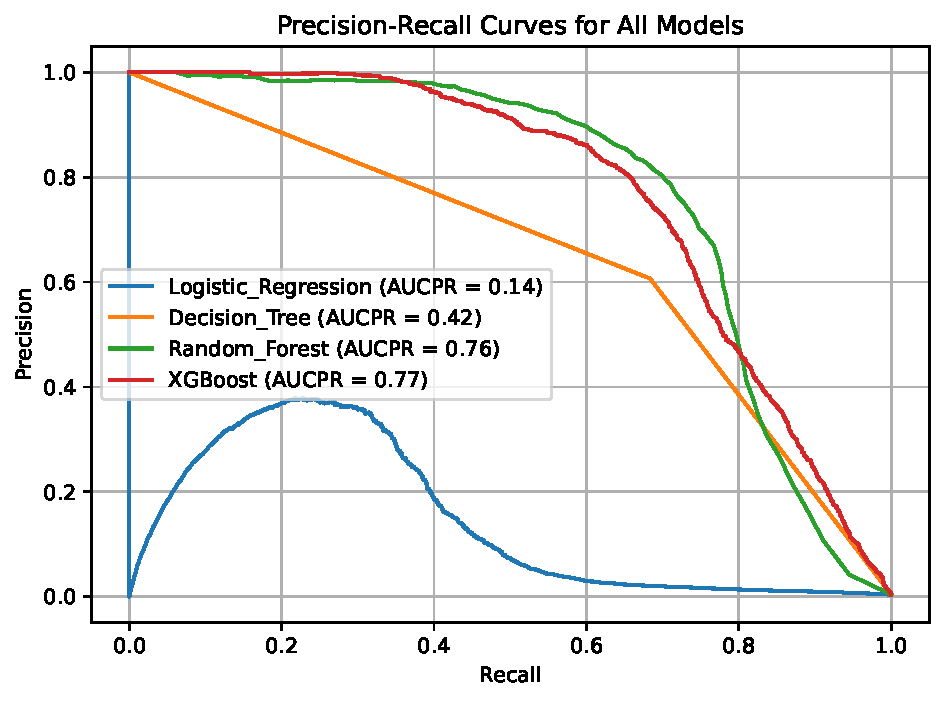
\includegraphics[width=0.7\columnwidth]{AUCPR Curve ML.pdf}
        \caption{Traditional ML}
        \label{fig:aucpr-ml}
    \end{subfigure}
    
    \vspace{0.3cm}
    
    \begin{subfigure}{\columnwidth}
        \centering
        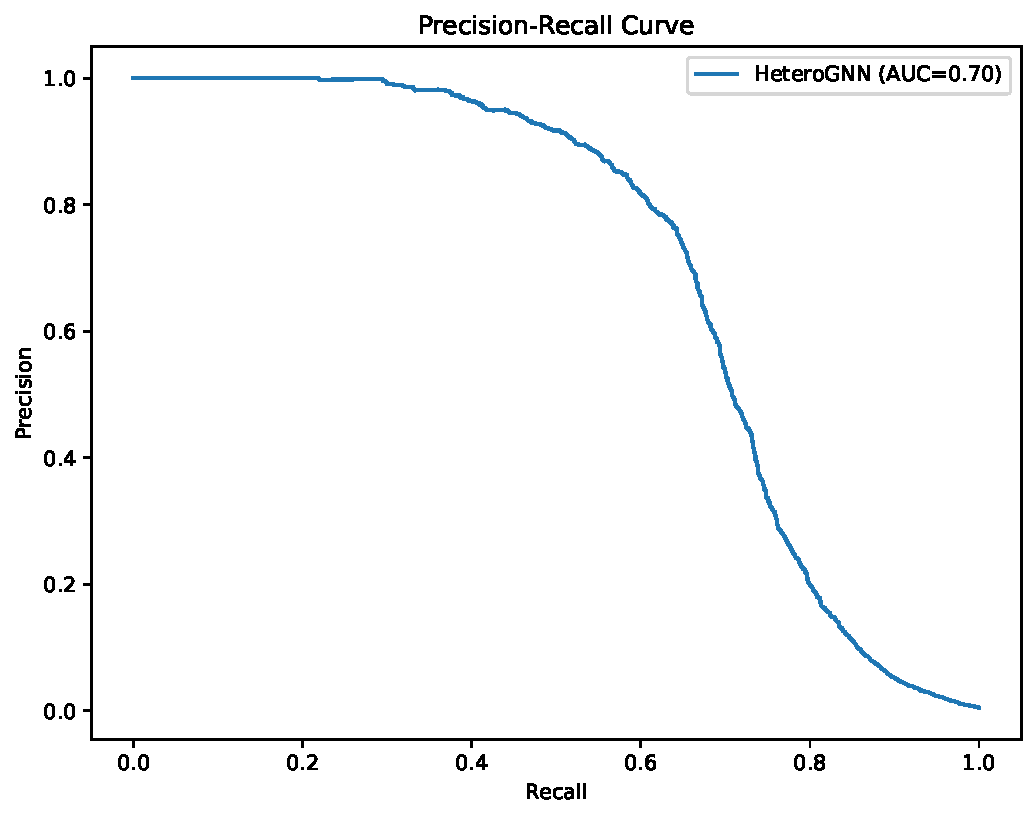
\includegraphics[width=0.7\columnwidth]{AUCPR GNN DS1.pdf}
        \caption{GNN Model}
        \label{fig:aucpr-gnn}
    \end{subfigure}
    
    \caption{Comparison of AUCPR Curves for Dataset 1.}
    \label{fig:aucpr-comparison-ds1}
\end{figure}

\begin{table}[htbp]
\caption{Performance Metrics of Different Methods for Dataset 1}
\centering
\begin{tabular}{lcccc}
\toprule
\textbf{Methods} & \textbf{Precision} & \textbf{Recall} & \textbf{F1-Score} & \textbf{AUCPR} \\
\midrule
XGBoost & 0.89 & 0.52 & 0.66 & 0.76 \\
Random Forest & 0.93 & 0.52 & 0.67 & 0.76 \\
Decision Tree & 0.60 & 0.68 & 0.64 & 0.41 \\
Logistic Regression & 0.00 & 0.00 & 0.00 & 0.13 \\
GNN & 0.73 & 0.65 & \textbf{0.68} & 0.47 \\
\bottomrule
\end{tabular}
\label{tab:metrics-ds1}
\end{table}


\subsection{Dataset 2 Results}

For Dataset 2, the GNN again demonstrates competitive performance against classical models, particularly in terms of F1-score and AUCPR, as presented in Fig.~\ref{fig:aucpr-comparison-ds2} and Table~\ref{tab:metrics-ds2}.

\begin{table}[htbp]
\caption{Performance Metrics of Different Methods for Dataset 2}
\centering
\begin{tabular}{lcccc}
\toprule
\textbf{Methods} & \textbf{Precision} & \textbf{Recall} & \textbf{F1-Score} & \textbf{AUCPR} \\
\midrule
XGBoost & 0.92 & 0.75 & \textbf{0.83} & 0.92 \\
Random Forest & 0.93 & 0.72 & 0.81 & 0.90 \\
Decision Tree & 0.66 & 0.80 & 0.72 & 0.57 \\
GNN & 0.90 & 0.75 & \textbf{0.82} & 0.73 \\
\bottomrule
\end{tabular}
\label{tab:metrics-ds2}
\end{table}

\begin{figure}[htbp]
    \centering
    \begin{subfigure}{\columnwidth}
        \centering
        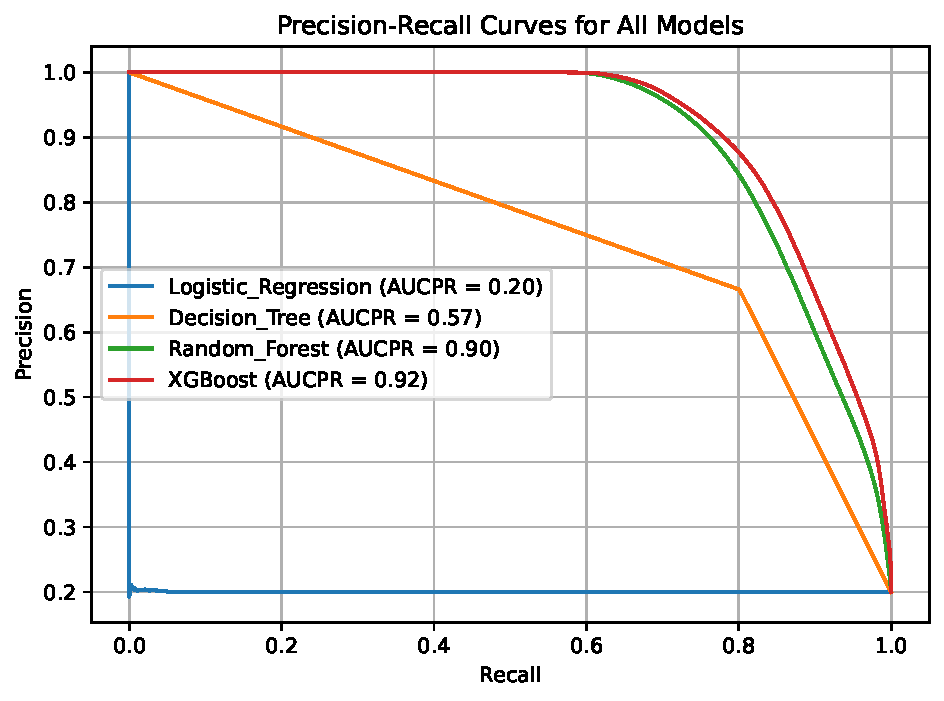
\includegraphics[width=0.7\columnwidth]{AUCPR Curve ML DS2.pdf}
        \caption{Traditional ML}
        \label{fig:aucpr-ml}
    \end{subfigure}
    
    \vspace{0.3cm}
    
    \begin{subfigure}{\columnwidth}
        \centering
        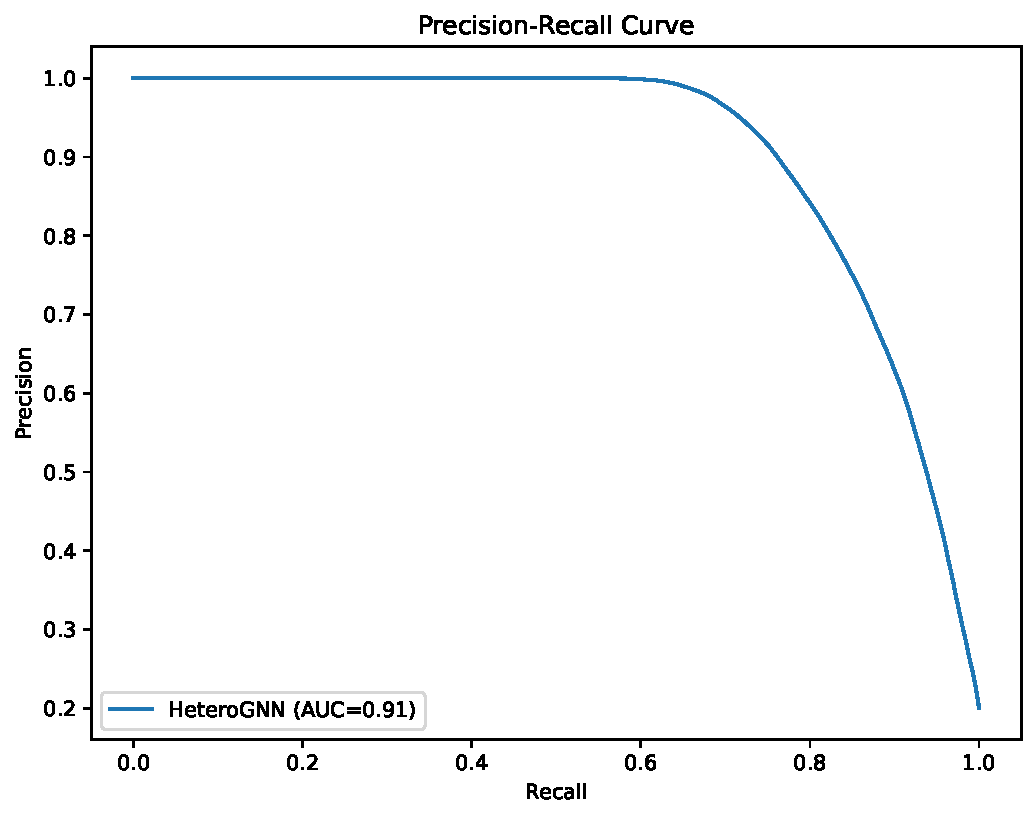
\includegraphics[width=0.7\columnwidth]{AUCPR GNN DS2.pdf}
        \caption{GNN Model}
        \label{fig:aucpr-gnn}
    \end{subfigure}
    
    \caption{Comparison of AUCPR Curves for Dataset 1.}
    \label{fig:aucpr-comparison-ds2}
\end{figure}


\newpage

\section{Conclusion}
In this study, we performed a comprehensive comparative analysis between classical machine learning models and Graph Neural Networks (GNNs) for the task of credit card fraud detection. Our approach leveraged both tabular and graph-based representations of financial transaction data to evaluate the effectiveness of these paradigms across two large datasets.

The results from Dataset 1 demonstrate that the GNN-based model outperforms classical ML models, particularly in settings where explicit features are limited and relational patterns dominate. The ability of graph architecture to exploit structural and contextual cues, through heterogeneous message passing between users, merchants, and transactions, resulted in superior fraud classification performance.

While the GNN still showed strong performance on Dataset 2, classical models like XGBoost and Random Forest slightly outperformed it. A key distinction in this dataset was the availability of numerous high-quality, logically meaningful features that classical models could leverage effectively without relying on inter-node relationships. This contrast highlights a critical insight: GNNs are most advantageous in environments where feature engineering is constrained but relational data is rich, whereas classical models retain their strength when abundant, well-engineered features are present.

Overall, our findings affirm that GNNs are a powerful and scalable alternative to traditional models, particularly suited for fraud detection systems embedded in relationally complex environments. 


\section{Future Scope}
Future work may explore hybrid models that combine GNN embeddings with classical classifiers or apply explainable GNNs to enhance trust and interpretability in financial applications.

\section{Data Availability}
The data supporting the findings of this study are
available on Kaggle at \href{https://www.kaggle.com/datasets/kartik2112/fraud-detection/data}{www.kaggle.com/datasets/kartik2112/fraud-detection} and at \href{https://www.kaggle.com/datasets/ismetsemedov/transactions/data}{www.kaggle.com/datasets/ismetsemedov/transactions/} .

\section{Conflict of Interest}
I hereby certify that to the best of my knowledge,
the authors have no relevant financial or non-financial interests to disclose. The authors have no conflict of interest to declare that are relevant to the content of this article. All authors certify that they have no affiliations with or involvement in any organization or entity with
any financial interest or non-financial interest in the subject matter or materials discussed in this manuscript. The authors have no financial or proprietary interests in any material discussed in this article.

\begin{thebibliography}{99}

\bibitem{chaudhary2012review}
K. Chaudhary, J. Yadav, and B. Mallick, Dept. of Computer Science, GCET, Greater Noida, India. ``A review of fraud detection techniques: credit card,'' 2012. \href{https://d1wqtxts1xzle7.cloudfront.net/74530838/pxc3878991-libre.pdf?1636648580=&response-content-disposition=inline%3B+filename%3DA_review_of_Fraud_Detection_Techniques_C.pdf&Expires=1745510471&Signature=YcBJAmZm~XRNUlp0ZgYoKpNDj1OgjLYGHCEFPXtB6xIspkQyxp0Oh7gMxJJ20hWEDdy0OLL2yxZmrSQRyy3IkygJQ7Njt1JwyTW8qJirZ8ClKnKnM0ZkTDV8JVlHMlWrQjTc~nTOQ9zZZhLtQwaCDuW~pC27fYhbgKqHqUYx-6YehYvANl0zcfTLy5tI~yA89LNvAxVUbME66VOAX6CBtFonZ~ha6Gp-FRyvAsII54aLdh5-ymGuMELYDjWtO-pFAPyJDAsd8afdq~sPlDUJwZD-E5-aYqeszHpCrGBC0RtCY8dNGhuxgnP7teBz2oXwfR5YwYGo~gMcQabIH2KPhg__&Key-Pair-Id=APKAJLOHF5GGSLRBV4ZA}{cloudfront.net/...libre.pdf}

\bibitem{xuan2018random}
Xuan, Shiyang and Liu, Guanjun and Li, Zhenchuan and Zheng, Lutao and Wang, Shuo and Jiang, Changjun. ``Random forest for credit card fraud detection,'' 2018.\\
\href{https://ieeexplore.ieee.org/abstract/document/8361343}{https://ieeexplore.ieee.org/abstract/document/8361343}

\bibitem{sailusha2020ml}
Sailusha, Ruttala and Gnaneswar, V. and Ramesh, R. and Rao, G. Ramakoteswara. ``Credit card fraud detection using machine learning,'' 2020.\\
\href{https://ieeexplore.ieee.org/abstract/document/9121114}{https://ieeexplore.ieee.org/abstract/document/9121114}


\bibitem{awoyemi2017comparative}
Awoyemi, John O. and Adetunmbi, Adebayo O. and Oluwadare, Samuel A. ``Credit card fraud detection using machine learning techniques: A comparative analysis,'' 2017.\\
\href{https://ieeexplore.ieee.org/abstract/document/8123782?casa_token=agN3nFNpjkkAAAAA:Y0GKH4PXeCQjLyvXOHGsm9uILsQ40S1yi6Dw_p4rrsvVLYY78ronmk5yZS31tHM5uI7x7BPu}{https://ieeexplore.ieee.org/abstract/document/8123782/...}

\bibitem{dataset2}
Ismat Samadov, Soonhyeong Kwon, Aadya Singh. ``Transactions,'' 2020.\\
\href{https://www.kaggle.com/datasets/ismetsemedov/transactions/data}{https://www.kaggle.com/datasets/ismetsemedov/transactions/data}

\bibitem{dataset1}
Kartik Shenoy, Brandon Harris. ``Credit card transactions fraud detection dataset,'' 2020.\\
\href{https://www.kaggle.com/datasets/kartik2112/fraud-detection/data}{https://www.kaggle.com/datasets/kartik2112/fraud-detection/data}

\bibitem{ieee1297040}
Yufeng Kou and Chang-Tien Lu and Sirwongwattana, S. and Yo-Ping Huang. ``Survey of fraud detection techniques,'' 2004.\\
\href{https://ieeexplore.ieee.org/abstract/document/1297040}{https://ieeexplore.ieee.org/abstract/document/1297040}


\bibitem{IEEE9719580}
Abdulghani, Ahmed Qasim and UCAN, Osman Nuri and Alheeti, Khattab M. Ali. ``Credit card fraud detection using XGBoost algorithm,'' 2021.\\
\href{https://ieeexplore.ieee.org/abstract/document/9719580}{https://ieeexplore.ieee.org/abstract/document/9719580}

\bibitem{IEEE9667674}
Tan, Runnan and Tan, Qingfeng and Zhang, Peng and Li, Zhao. ``Graph neural network for ethereum fraud detection,'' 2021.\\
\href{https://ieeexplore.ieee.org/abstract/document/9667674}{https://ieeexplore.ieee.org/abstract/document/9667674}

\bibitem{IEEE9906987}
Kim, Hwan and Lee, Byung Suk and Shin, Won-Yong and Lim, Sungsu. ``Graph anomaly detection with graph neural networks: current status and challenges,'' 2022.\\
\href{https://ieeexplore.ieee.org/document/9906987}{https://ieeexplore.ieee.org/document/9906987}


\bibitem{paper3}
C. Leo, ``Deep dive into graph neural networks: break down the math, explore message passing mechanisms, and build a GCN from scratch in Python,'' 2024. [Online]. Available: \href{https://medium.com/@cristianleo120/the-math-behind-graph-neural-networks-3427c16570d0}{https://medium.com/@cristianleo120/...}
\bibitem{dgl}
Amazon Web Services AI Shanghai Lablet et al., ``Deep graph library package,'' 2024. [Online]. Available: \href{https://www.dgl.ai/}{https://www.dgl.ai/}

\bibitem{PyG}
PyTorch Geometric, ``Blogs and tutorials,'' 2022. [Online]. Available: \href{https://pyg.org/blogs-and-tutorials}{https://pyg.org/blogs-and-tutorials}

\bibitem{paper1}
Z. Wu et al., ``A comprehensive survey on graph neural networks,'' 2019. [Online]. Available: \href{https://arxiv.org/pdf/1901.00596}{https://arxiv.org/pdf/1901.00596}

\bibitem{Math}
R. Anand, ``Math behind graph neural networks,'' 2022. [Online]. Available: \href{https://rish-16.github.io/posts/gnn-math/}{https://rish-16.github.io/posts/gnn-math/}


\bibitem{paper2}
Sing Kwan NG and Anthony TAING as part of the Stanford CS224W course project. ``Fraud detection with graph attention networks,'' 2022.\\
\href{https://medium.com/stanford-cs224w/fraud-detection-with-gat-edac49bda1a0}{https://medium.com/stanford-cs224w/...}

\bibitem{GNNbasic}
Omar Hussein, AI Engineer. ``Graph neural networks series,'' 2022.\\
\href{https://medium.com/the-modern-scientist/graph-neural-networks-series-part-2-graph-statistics-4f271857ec70}{https://medium.com/the-modern-scientist/...}

\bibitem{amazonPaper}
Amazon. ``Build a GNN-based real-time fraud detection solution using Amazon SageMaker, Amazon Neptune, and the deep graph library,'' 2023.\\
\href{https://aws.amazon.com/blogs/machine-learning/build-a-gnn-based-real-time-fraud-detection-solution-using-amazon-sagemaker-amazon-neptune-and-the-deep-graph-library/?utm_source=chatgpt.com}{https://aws.amazon.com/blogs/machine-learning/...}


\bibitem{paper5}
Dawei Cheng, Yao Zou, Sheng Xiang, Changjun Jiang; Department of Computer Science and Technology, Tongji University, Shanghai, China; Shanghai Artificial Intelligence Laboratory, Shanghai, China; National Collaborative Innovation Center for Internet Financial Security, Shanghai, China; AAII, University of Technology Sydney, Australia. ``Graph neural networks for financial fraud detection: a review,'' 2024.\\
\href{https://arxiv.org/pdf/2411.05815}{https://arxiv.org/pdf/2411.05815}

\bibitem{data_generation}
Ismat-Samadov. ``Synthetic data generator,'' 2024.\\
\href{https://github.com/Ismat-Samadov/fraud_detection/blob/main/data_gen.py}{https://github.com/Ismat-Samadov/fraud_detection/blob/main/data_gen.py}


\bibitem{cheng2025gnnreview}
Cheng, D., Zou, Y., Xiang, S. et al. ``Graph neural networks for financial fraud detection: a review,'' 2025.\\
\href{https://link.springer.com/article/10.1007/s11704-024-40474-y#Abs1}{https://link.springer.com/article/10.1007/s11704-024-40474-y#Abs1}


\bibitem{IEEE10689393}
Khaled Alarfaj, Fawaz and Shahzadi, Shabnam. ``Enhancing fraud detection in banking with deep learning: graph neural networks and autoencoders for real-time credit card fraud prevention,'' 2025.\\
\href{https://ieeexplore.ieee.org/abstract/document/10689393}{https://ieeexplore.ieee.org/abstract/document/10689393}


\bibitem{paper4}
Jianian Wang, Sheng Zhang, Yanghua Xiao, and Rui Song, Department of Statistics, North Carolina State University; School of Computer Science, Fudan University. ``A review on graph neural network methods in financial applications,'' 2022.\\
\href{https://arxiv.org/pdf/2111.15367}{https://arxiv.org/pdf/2111.15367}

\bibitem{paper5}
Dawei Cheng, Yao Zou, Sheng Xiang, Changjun Jiang; Department of Computer Science and Technology, Tongji University, Shanghai, China; Shanghai Artificial Intelligence Laboratory, Shanghai, China; National Collaborative Innovation Center for Internet Financial Security, Shanghai, China; AAII, University of Technology Sydney, Australia. ``Graph neural networks for financial fraud detection: A review,'' 2024.\\
\href{https://arxiv.org/pdf/2411.05815}{https://arxiv.org/pdf/2411.05815}


\bibitem{prcurve}
Doug Steen, Data Analyst, Geologist, Data Science \& ML Enthusiast. \textit{Precision-Recall curves}. (2020).\\
\url{https://medium.com/@douglaspsteen/precision-recall-curves-d32e5b290248}


\bibitem{IEEE9736204}
Liu, GuanJun and Tang, Jing and Tian, Yue and Wang, Jiacun. ``Graph neural network for credit card fraud detection,'' 2021.\\
\href{https://ieeexplore.ieee.org/abstract/document/9736204}{https://ieeexplore.ieee.org/abstract/document/9736204}


\bibitem{IEEE9736204}
Liu, GuanJun and Tang, Jing and Tian, Yue and Wang, Jiacun. ``Graph neural network for credit card fraud detection,'' 2021.\\
\href{https://ieeexplore.ieee.org/abstract/document/9736204}{https://ieeexplore.ieee.org/abstract/document/9736204}


\end{thebibliography}
\end{document}
